\documentclass[11pt,class=report,crop=false]{standalone}
\usepackage{exo7sv}

\begin{document}

%%%%%%%%%%%%%%%%%%%%%%%%%%%%%%%%%%%%%%%%%%%%%%%%%%%%%%%%%%%%%%%%%%%%%%
%%%%%%%%%%%%%%%%%%%%%%%%%%%%%%%%%%%%%%%%%%%%%%%%%%%%%%%%%%%%%%%%%%%%%%

\section*{Longueur, aire, volume}


\setcounterexo{28}
% exercice 29
\exercice{}
\enonce
    On remplit d'eau un bol hémisphérique, de rayon $r$ (en {cm}).
    \begin{center}
       \begin{tikzpicture}
    \tikzstyle{point} = [circle,inner sep=1pt,fill, draw]
    \begin{scope}[xmin=-2,xmax=3,ymin=-2.1,ymax=2.1]
        % les axes
    \draw[thick, ->] (\xmin,0) -- (\xmax,0);
    \draw[thick, ->] (0,\ymin) -- (0,\ymax);
       % \axes
        \node[right] at (\xmax, 0) {$x$};
        \node[above] at (0, \ymax) {$f(x)$};
        % le bol obtenu par révolution
        \draw[blue, opacity=.5] (2,0) circle [x radius=.5, y radius=2];
        \draw[thin, opacity=.5] (2,2) -- (2,0);
        \draw[very thick, blue] (2,2) arc (90:270:2);
        % l'origine
        \path (0,0) node[point]{} node[below left] {$0$};
        % le triangle rectangle
        \draw[red] (1,0) node[point]{} node[below] {$x$} -- (1,1.732) -- (2,0) node[point]{} node[below] {$r$} -- cycle;
        % la valeur de f(x)
        \draw[opacity=0.35] (1,1.732) -- (0,1.732);
        \draw[decorate,decoration=brace, red] (-0.1,0) -- (-0.1,1.732) node[left=2, pos=0.5, scale=0.7] {$\sqrt{r^{2}-(x-r)^{2}}$};
    \end{scope}
\end{tikzpicture}

    \end{center}
    Un tel bol est obtenu par rotation autour de l'axe $x$ de la courbe représentant $f(x)=\sqrt{r^{2}-(x-r)^{2}}$ pour $x \in [0,r]$.
    \begin{enumerate}
        \item Montrer que, s'il est rempli jusqu'à une hauteur $h$ (en {cm}), le bol contient (en {cm$^{3}$})
        $$
            V(h)= \frac{1}{3}\pi h^{2}(3r-h).
        $$
        \item En déduire le volume d'eau que peut contenir le bol.
        \item Écrire l'équation déterminant à quelle hauteur le bol sera à moitié plein.
        \item Le bol fait 5 centimètres de rayon et l'eau coule à un débit de {20}~{cm$^3$/s}.

        \noindent
        \begin{minipage}{9.5cm}
            \begin{enumerate}
                \item Combien de temps faudra-t-il pour que la hauteur de l'eau passe de 2 centimètres à 4 centimètres ?
                \item Soit $h(t)$ la hauteur (en {cm}) au temps $t$ (en {s}). Montrer que
                $$
                    h'(t)(10\pi h(t)-\pi h^{2}(t)) = 20.
                $$
                \item A quelle vitesse le niveau de l'eau monte-t-il s'il y a déjà 2 centimètres d'eau au fond ?
            \end{enumerate}
        \end{minipage}
        \begin{minipage}{7cm}
            \vspace{2mm}\hfill
            \begin{tikzpicture}
    % l'eau qui coule
    \fill[decoration={coil,aspect=1, amplitude=.35}, blue, opacity=.35] decorate{(-.25,3.77) -- (-.25,1)} arc [x radius=.25, y radius=.125, start angle=-180, end angle=0] decorate{-- (.25,3.77)};
    % le robinet (en SVG)
    \filldraw[yscale=-1, scale=3, yshift=-35] (0,0) svg "M -4.37,-12.47 C -4.00,-12.46 -4.00,-12.11 -4.00,-11.83 C -3.93,-11.90 -3.84,-11.95 -3.73,-11.95 C -3.03,-11.95 -1.64,-11.95 -0.95,-11.95 C -0.43,-11.94 -0.43,-10.99 -0.95,-10.98 C -1.64,-10.98 -3.03,-10.98 -3.73,-10.98 C -3.84,-10.98 -3.93,-11.02 -4.00,-11.09 C -4.00,-10.82 -4.00,-10.28 -4.00,-10.01 C -3.21,-9.78 -3.43,-8.71 -3.43,-8.07 C -2.86,-8.07 -2.20,-8.00 -2.19,-7.27 C -2.19,-7.10 -2.19,-6.76 -2.19,-6.58 C -1.57,-6.58 -0.31,-6.58 0.31,-6.58 C 1.06,-6.58 1.68,-6.02 1.76,-5.30 C 1.77,-5.30 1.77,-5.30 1.77,-5.30 C 1.77,-4.40 1.77,-2.61 1.77,-1.72 C 2.31,-1.72 2.86,-1.55 2.86,-0.90 C 2.86,-0.45 2.81,-0.44 2.81,-0.44 C 1.41,0.00 -1.59,0.00 -2.93,-0.44 C -2.93,-0.44 -2.98,-0.45 -2.98,-0.90 C -2.98,-1.35 -2.60,-1.83 -2.16,-1.72 C -2.11,-1.72 -1.99,-1.72 -1.94,-1.72 C -1.94,-2.20 -1.94,-3.18 -1.94,-3.66 C -4.08,-3.66 -8.38,-3.66 -10.52,-3.66 C -10.52,-3.17 -10.52,-2.18 -10.52,-1.69 C -10.53,-0.82 -11.43,-0.89 -12.05,-0.89 C -12.59,-3.00 -12.59,-7.00 -12.05,-9.20 C -11.84,-9.20 -11.50,-9.20 -11.31,-9.20 C -10.87,-9.20 -10.66,-8.83 -10.52,-8.41 C -10.52,-7.95 -10.52,-7.04 -10.52,-6.58 C -9.53,-6.58 -7.54,-6.58 -6.55,-6.58 C -6.55,-7.20 -6.60,-8.06 -5.75,-8.07 C -5.64,-8.07 -5.42,-8.07 -5.31,-8.07 C -5.31,-8.71 -5.52,-9.78 -4.74,-10.01 C -4.74,-10.28 -4.74,-10.82 -4.74,-11.10 C -4.81,-11.02 -4.90,-10.98 -5.01,-10.98 C -5.71,-10.98 -7.10,-10.98 -7.79,-10.98 C -8.31,-10.98 -8.31,-11.94 -7.79,-11.95 C -7.10,-11.95 -5.71,-11.95 -5.01,-11.95 C -4.90,-11.95 -4.81,-11.90 -4.74,-11.83 C -4.74,-12.10 -4.74,-12.47 -4.37,-12.47 Z";
    % l'axe des x avec l'origine 0
    \draw[thick, ->, opacity=.5] (0,-.5) -- (0,3) node[above] {$x$};
    \draw[opacity=.5] (0,0) node[circle,inner sep=1pt,fill, draw]{} node[below left]{$0$};
    % le bol
    \draw[very thick, blue] (-2,2) arc (-180:0:2) (0,2) circle[x radius=2, y radius=.5];
    % l'eau dans le bol
    \draw[thin, blue, opacity=0.7] (0,1) circle[x radius=1.732, y radius=.433];
    \fill[blue, opacity=0.2] (0,1) circle[x radius=1.732, y radius=.433];
    \fill[blue, opacity=0.1] (-1.732,1) arc (-150:-30:2) arc [x radius=1.732, y radius=.433, start angle=0, end angle=180];
    % les mesures
    \begin{scope}[red]
        \draw (0.5,0) -- (3,0);
        \draw (1.8,1) -- (2.5,1);
        \draw (2.1,2) -- (3,2);
        \draw[-latex] (.35,3.5) -- (.35,2.7) node[pos=.5, right]{20 cm$^3$/s};
        \draw[latex-latex] (2.3,0) -- (2.3,1) node[pos=.5, left]{$h$};
        \draw[latex-latex] (2.8,0) -- (2.8,2) node[pos=.5, right]{5 cm};
    \end{scope}
\end{tikzpicture}

        \end{minipage}
    \end{enumerate}
\finenonce

\indication
\sauteligne
\begin{enumerate}
\item $V(h) = \int_0^h \pi f(x)^2 \dd x$
\item Calculer $V(r)$.
\item L'équation est \og{}$V(h)$ est égale à la moitié de $V(r)$\fg{}. On ne demande pas de trouver le $h$ solution de cette équation.
\item 
\begin{enumerate}
	\item Calculer $V(4)-V(2)$. Le débit est donné par $\text{débit} = \frac{\text{volume}}{\text{temps}}$.
	\item Le débit à un instant $t$ est aussi la dérivée du volume par rapport au temps, ici c'est donc $\big( V(h(t)) \big) '$.
	\item La vitesse de montée de l'eau est donnée par $h'(t)$ que l'on peut calculer en utilisant la question précédente avec ici $h(t)=2$.
\end{enumerate}
\end{enumerate}
	

\finindication

\correction

\video{5qY8nVnGe8k}

\sauteligne
\begin{enumerate}
  \item 
\begin{align*}
V(h) 
  &= \int_0^h \pi f(x)^2 \dd x \\
  &= \int_0^h \pi\big( r^2 - (x-r)^2\big) \dd x \\
  &= \pi\int_0^h (2xr-x^2) \dd x \\
  &= \pi\left[ x^2r-\frac{x^3}{3} \right]_0^h \\
  &= \pi\left(h^2r-\frac{h^3}{3} \right) \\
\end{align*}
  \item 
$$V(r) =  \pi\left(r^2r-\frac{r^3}{3} \right) = \frac23 \pi r^3$$

  \item L'équation est $V(h) = \frac12 V(r)$, c'est-à-dire
$$\pi h^2\left(r-\frac{h}{3} \right) = \frac12\cdot \frac23 \pi r^3$$
ou encore
$$h^2(3r-h) = r^3.$$
On ne demande pas de résoudre cette équation.
  \item 
  \begin{enumerate}
     \item Le volume d'eau nécessaire pour faire passer le niveau de $2$ à $4$ cm est :
$$V(4) - V(2) = \frac\pi3\big( 16(15-4) -4(15-2) \big) \simeq 128,8 \text{ cm$^3$}.$$
et le temps nécessaire est :
$$\text{temps} = \frac{\text{volume}}{\text{débit}} \simeq \frac{129,8}{20} \simeq 7 \text{ s}.$$

     \item Le débit est la dérivée du volume par rapport au temps, c'est-à-dire 
$$\text{débit} = \big( V(h(t)) \big)' = V'(h(t))\cdot h'(t) = \pi ( 2h(t)r-h(t)^2)h'(t).$$
Ici on obtient avec $r=5$ et débit de $20$ cm$^3$/s :
$$\pi ( 10h(t)-h(t)^2)h'(t) = 20.$$


     \item La vitesse du niveau de l'eau est la dérivée de $h$ par rapport au temps : $h'(t)$.
Par l'équation de la question précédente :
$$h'(t) = \frac{20}{\pi(10h(t)-h(t)^2)}.$$
On se place au temps $t_0$ où il y a déjà $2$ cm d'eau, alors $h(t_0)=2$
$$h'(t_0) = \frac{20}{\pi(10\cdot 2-2^2)} = \frac{20}{16\pi} \simeq 0,4 \text{ cm/s}.$$

  \end{enumerate}
\end{enumerate}
\fincorrection
\finexercice


% exercice 30
\exercice{}
\enonce
Soit $f$ une fonction continue sur le segment $[a,b]$.
\begin{enumerate}
	\item On admet que la longueur de la courbe d'équation $y=f(x)$ pour $x \in [a,b]$ est donnée par l'intégrale
	\begin{equation}
	L=\int_{a}^{b} \sqrt{1+f'(x)^{2}}\,dx. \label{long}
	\end{equation}
	\begin{enumerate}
		\item Soit $f$ une fonction constante: pour $x\in[a,b]$, $f(x)=c$. La formule (\ref{long}) donne-t-elle le résultat attendu?
		\item Soit $f$ une fonction affine: pour $x\in[a,b]$, $f(x)=kx+c$. Tracer le graphe de $f$. La formule (\ref{long}) donne-t-elle le résultat attendu?
		\item Calculer la longueur de la courbe d'équation $y=x^{\frac{3}{2}}$ pour $x \in [0,1]$.
	\end{enumerate}
	\item  Soit $f$ une fonction positive. On fait tourner la courbe d'équation $y=f(x)$ entre $x=a$ et $x=b$ autour de l'axe des $x$. On admet que l'aire de la surface ainsi obtenue est donnée par l'intégrale
	\begin{equation}
	A=\int_a ^b 2\pi f(x) \sqrt {(1+f'(x) ^2)}\,dx. \label{surf}
	\end{equation}
	\begin{enumerate}
		\item Soit $f$ une fonction constante. Quelle est la forme de l'objet obtenu? La formule (\ref{surf}) donne-t-elle le résultat attendu?
		\item Mêmes questions pour $f(x)= kx$ ($k > 0$) pour $x$ entre $0$ et $1$.
		\item Retrouver la formule de l'aire d'une sphère de rayon R.
	\end{enumerate}
\end{enumerate}
\finenonce

\indication
Une primitive de la fonction $ f(x) = u'(x) (u(x))^n $ est $ \frac{1}{n+1} 
(u(x))^{n+1} + C $, $ C \in \Rr $. 
\finindication

\correction

\video{OiQPXwFQ_0g}

\sauteligne
\begin{enumerate} 
	\item 
	\begin{enumerate} 
		\item 
		Soit $ f: [a, b] \rightarrow \Rr $, $ f(x) = c $ une fonction constante. 
		Alors la longueur de la courbe d'équation $ y = f(x) $, $ x \in [a, b] $, 
		est bien sûr $ b - a $. De plus, on a $ f'(x) = 0 $, $ x \in [a, b] $, et donc la formule donne :
		\begin{equation*} 
			\int_{a}^{b} \sqrt{1+f'(x)^{2}}\,dx = \int_a^b 1 \, dx = \left[x\right]_a^b 
			= b - a. 
		\end{equation*} 
		On retrouve bien le résultat attendu. 
		\item 
		Soit $ f(x) = kx + c $, $ x \in [a, b] $. Pour $ k = \frac{3}{2} $ and 
		$ a = 2 $ on a le graphe 
		\begin{center} 
			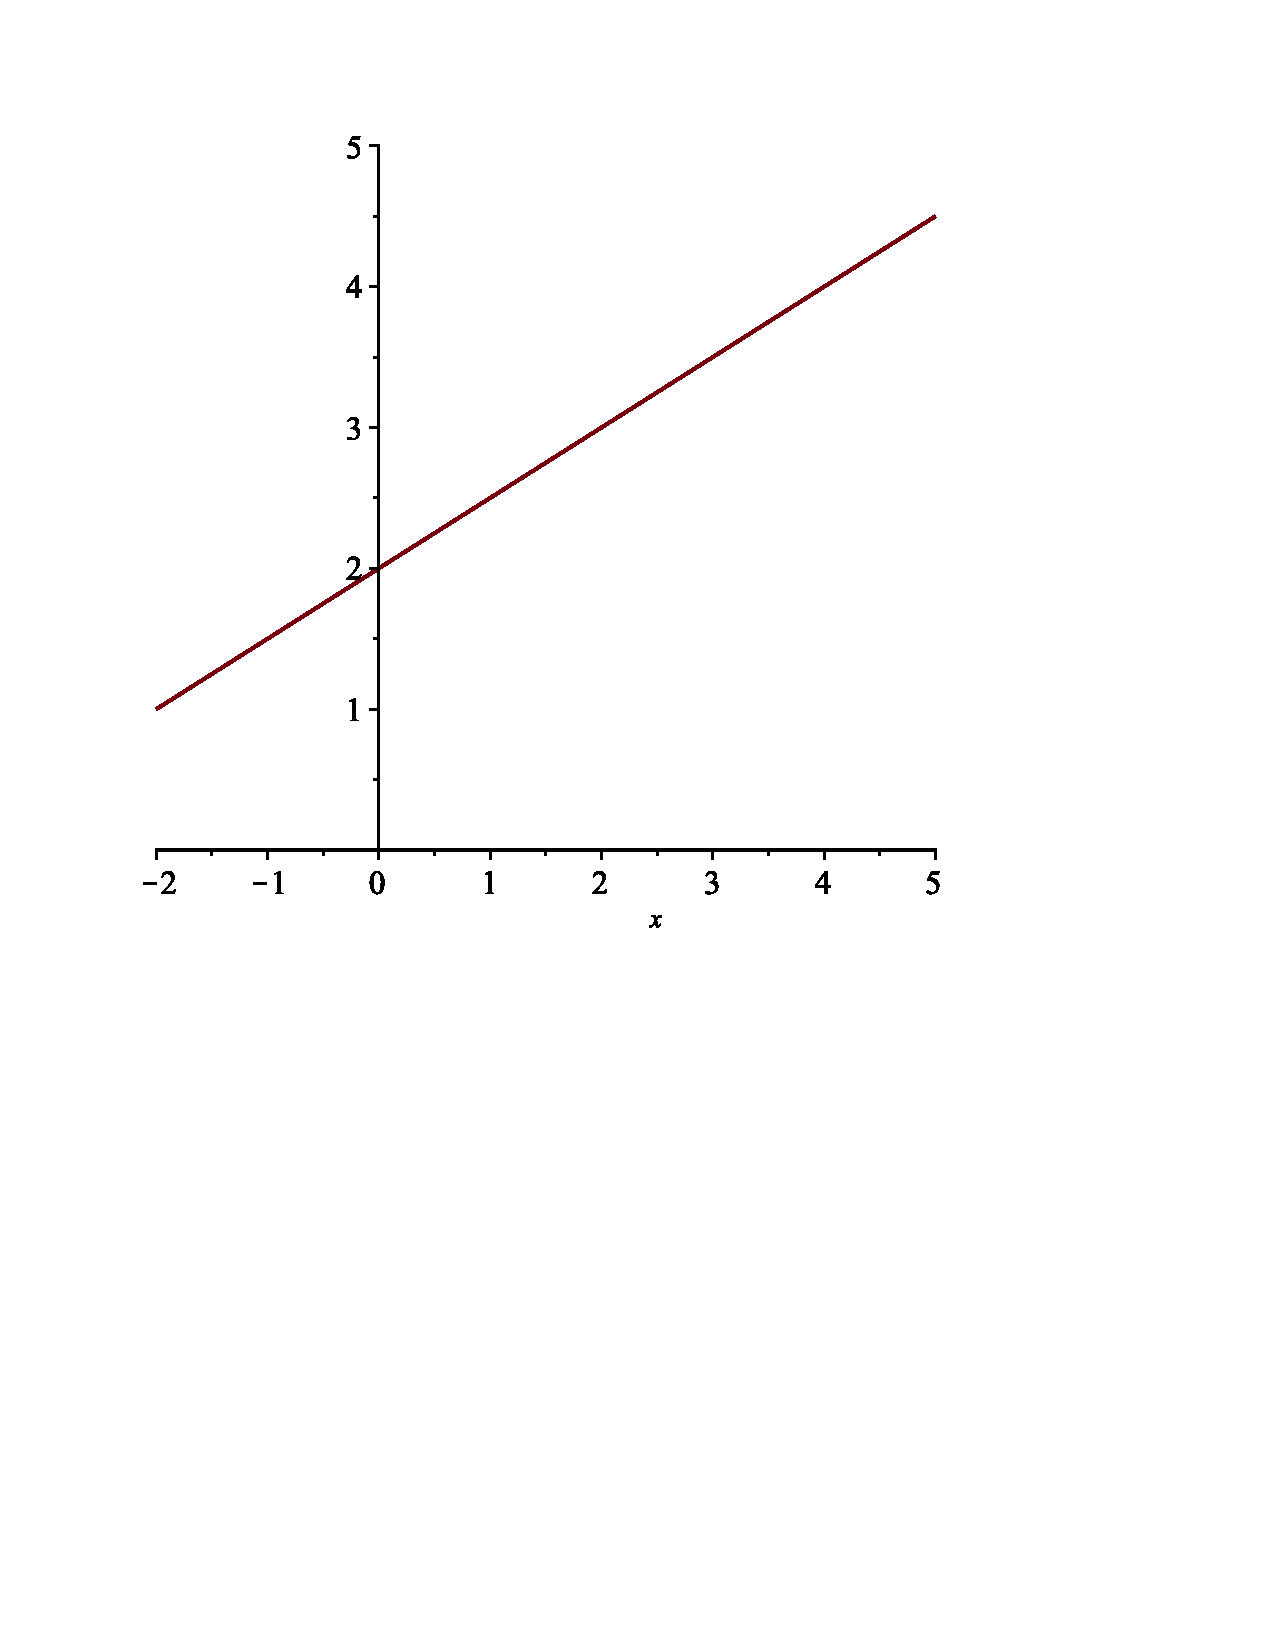
\includegraphics[height=10cm]{figures/plot4} 
		\end{center} 
		En utilisant le théorème de Phythagore on obtient que la longueur de 
		la courbe d'équation $ y = f(x) $, $ x \in [a, b] $, est donnée par 
		\begin{equation*} 
			\begin{split} 
				\sqrt{(f(b) - f(a))^2 + (b-a)^2} 
				&= \sqrt{(kb + c - (ka + c))^2 + (b-a)^2} 
				= \sqrt{(k(b-a))^2 + (b-a)^2} \\ 
				&= \sqrt{(b-a)^2 (k^2 + 1)} 
				= (b-a) \sqrt{k^2 + 1}. 
			\end{split} 
		\end{equation*} 
		De plus, on a $ f'(x) = k $, $ x \in [a, b] $, et d'après la formule (\ref{long}) :
		\begin{equation*} 
			\int_{a}^{b} \sqrt{1+f'(x)^{2}}\,dx = \int_a^b \sqrt{1 + k^2} \, dx 
			= \sqrt{1 + k^2} \int_a^b 1 \, dx
			= \sqrt{1 + k^2} \left[x\right]_a^b 
			= \sqrt{1 + k^2} (b - a). 
		\end{equation*} 
		Ainsi la formule donne bien le résultat attendu. 
		\item 
		Comme la dérivée de la fonction $ f(x) = x^{\frac{3}{2}} $ est $ f'(x) = 
		\frac{3}{2} x^{\frac{1}{2}} $ la formule (\ref{long}) implique 
		\begin{equation*} 
			\begin{split} 
				L &= \int_0^1 \sqrt{1 + \tfrac{9}{4} x} \, dx 
				= \frac{4}{9} \int_0^1 \frac{9}{4} \, \sqrt{1 + \tfrac{9}{4} x} \, dx 
				= \frac{4}{9} \left[\frac{2}{3} \left(1 + \frac{9}{4} x\right)^{\frac{3}{2}}\right]_0^1 
				= \frac{8}{27} \left(\left(1 + \frac{9}{4}\right)^{\frac{3}{2}} - 1\right) \\ 
				&= \frac{8}{27} \left(\left(\frac{13}{4}\right)^{\frac{3}{2}} - 1\right). 
			\end{split} 
		\end{equation*} 
	\end{enumerate} 
	\item 
	\begin{enumerate} 
		\item 
		Si $ f(x) = c $, $ x \in [a, b] $, $ c \in \Rr $, alors on obtient un 
		cylindre de rayon $ r = c $ et hauteur $ h = b - a $. Donc l'aire de la 
		surface est $ A = 2 \pi c (b-a) $. Comme $ f'(x) = 0 $, $ x \in [a, b] $, 
		on obtient en utilisant la formule (\ref{surf}) :
		\begin{equation*} 
			A = \int_a ^b 2\pi c \sqrt {1}\,dx 
			= 2\pi c \int_a^b 1 \, dx = 2\pi c \left[x\right]_a^b = 2\pi c (b-a) 
		\end{equation*} 
		et la formule donne le résultat attendu. 
		\item 
		Si $ f(x) = kx $, $ x \in [0, 1] $, $ k \in \Rr $, alors on obtient un 
		c\^one de rayon $ r = f(1) = k $ et hauteur $ h = 1 $. Donc l'aire de 
		la surface est $ A = \pi k \sqrt{1 + k^2} $. Comme $ f'(x) = k $, $ x 
		\in [0, 1] $, on obtient en utilisant la formule (\ref{surf}) 
		\begin{equation*} 
			A = \int_0^1 2 \pi kx \sqrt{1 + k^2}\,dx 
			= 2 \pi k \sqrt{1 + k^2} \int_0^1 x \, dx 
			= 2 \pi k \sqrt{1 + k^2} \left[\frac{1}{2} x^2\right]_0^1 
			= \pi k \sqrt{1 + k^2} 
		\end{equation*} 
		et la formule donne le résultat attendu. 
		\item 
		On obtient une sphère de rayon $ R $ si on fait tourner la courbe d'équation 
		$ y = f(x) = \sqrt{R^2 - x^2} $, $ x \in [-R, R] $, autour de l'axe des $ x $. 
		Comme $ f'(x) = \frac{-x}{\sqrt{R^2 - x^2}} $ la formule (\ref{surf}) donne 
		\begin{equation*} 
			\begin{split} 
				A 
				&= \int_{-R}^{R} 2 \pi \sqrt{R^2 - x^2} \sqrt{1 + \frac{x^2}{R^2 - x^2}} \, dx 
				= 2 \pi \int_{-R}^{R} \sqrt{R^2 - x^2} \sqrt{\frac{R^2 - x^2 + x^2}{R^2 - x^2}} \, dx \\ 
				&= 2 \pi \int_{-R}^{R} \sqrt{R^2} \, dx 
				= 2 \pi R \int_{-R}^{R} 1 \, dx 
				= 2 \pi R \left[x\right]_{-R}^{R} 
				= 2 \pi R \cdot 2 R 
				= 4 \pi R^2. 
			\end{split} 
		\end{equation*} 
	\end{enumerate} 
\end{enumerate} 
\fincorrection
\finexercice



\end{document}